% ------------------------------------------------------------------------------
% TYPO3 CMS 8.6 - What's New - Chapter "Backend User Interface" (Italian Version)
%
% @author	Michael Schams <schams.net>
% @license	Creative Commons BY-NC-SA 3.0
% @link		http://typo3.org/download/release-notes/whats-new/
% @language	English
% ------------------------------------------------------------------------------
% LTXE-CHAPTER-UID:		07b25346-95b1df21-a6ebe09a-49f53f41
% LTXE-CHAPTER-NAME:	Backend User Interface
% ------------------------------------------------------------------------------

\section{Interfaccia utente Backend}
\begin{frame}[fragile]
	\frametitle{Interfaccia utente Backend}

	\begin{center}\huge{Capitolo 1:}\end{center}
	\begin{center}\huge{\color{typo3darkgrey}\textbf{Interfaccia utente Backend}}\end{center}

\end{frame}

% ------------------------------------------------------------------------------
% LTXE-SLIDE-START
% LTXE-SLIDE-UID:		aa2f8c14-932ba2aa-0586f968-60a0de68
% LTXE-SLIDE-ORIGIN:	4141a9cc-46da51df-9dd87a8b-9b15ac29 English
% LTXE-SLIDE-TITLE:		#12211: Scheduler Page Browser
% LTXE-SLIDE-REFERENCE:	!Feature: #12211 - Usability: Scheduler provide page browser to choose start page
% ------------------------------------------------------------------------------
\begin{frame}[fragile]
	\frametitle{Interfaccia utente Backend}
	\framesubtitle{Scheduler Page Browser}

	Per migliorare l'usabilità del processo dello scheduler \textbf{EXT:linkvalidator},
	è stata aggiunta la pagina di navigazione per selezionare la pagina di partenza.

	\begin{figure}\vspace{-0.2cm}
		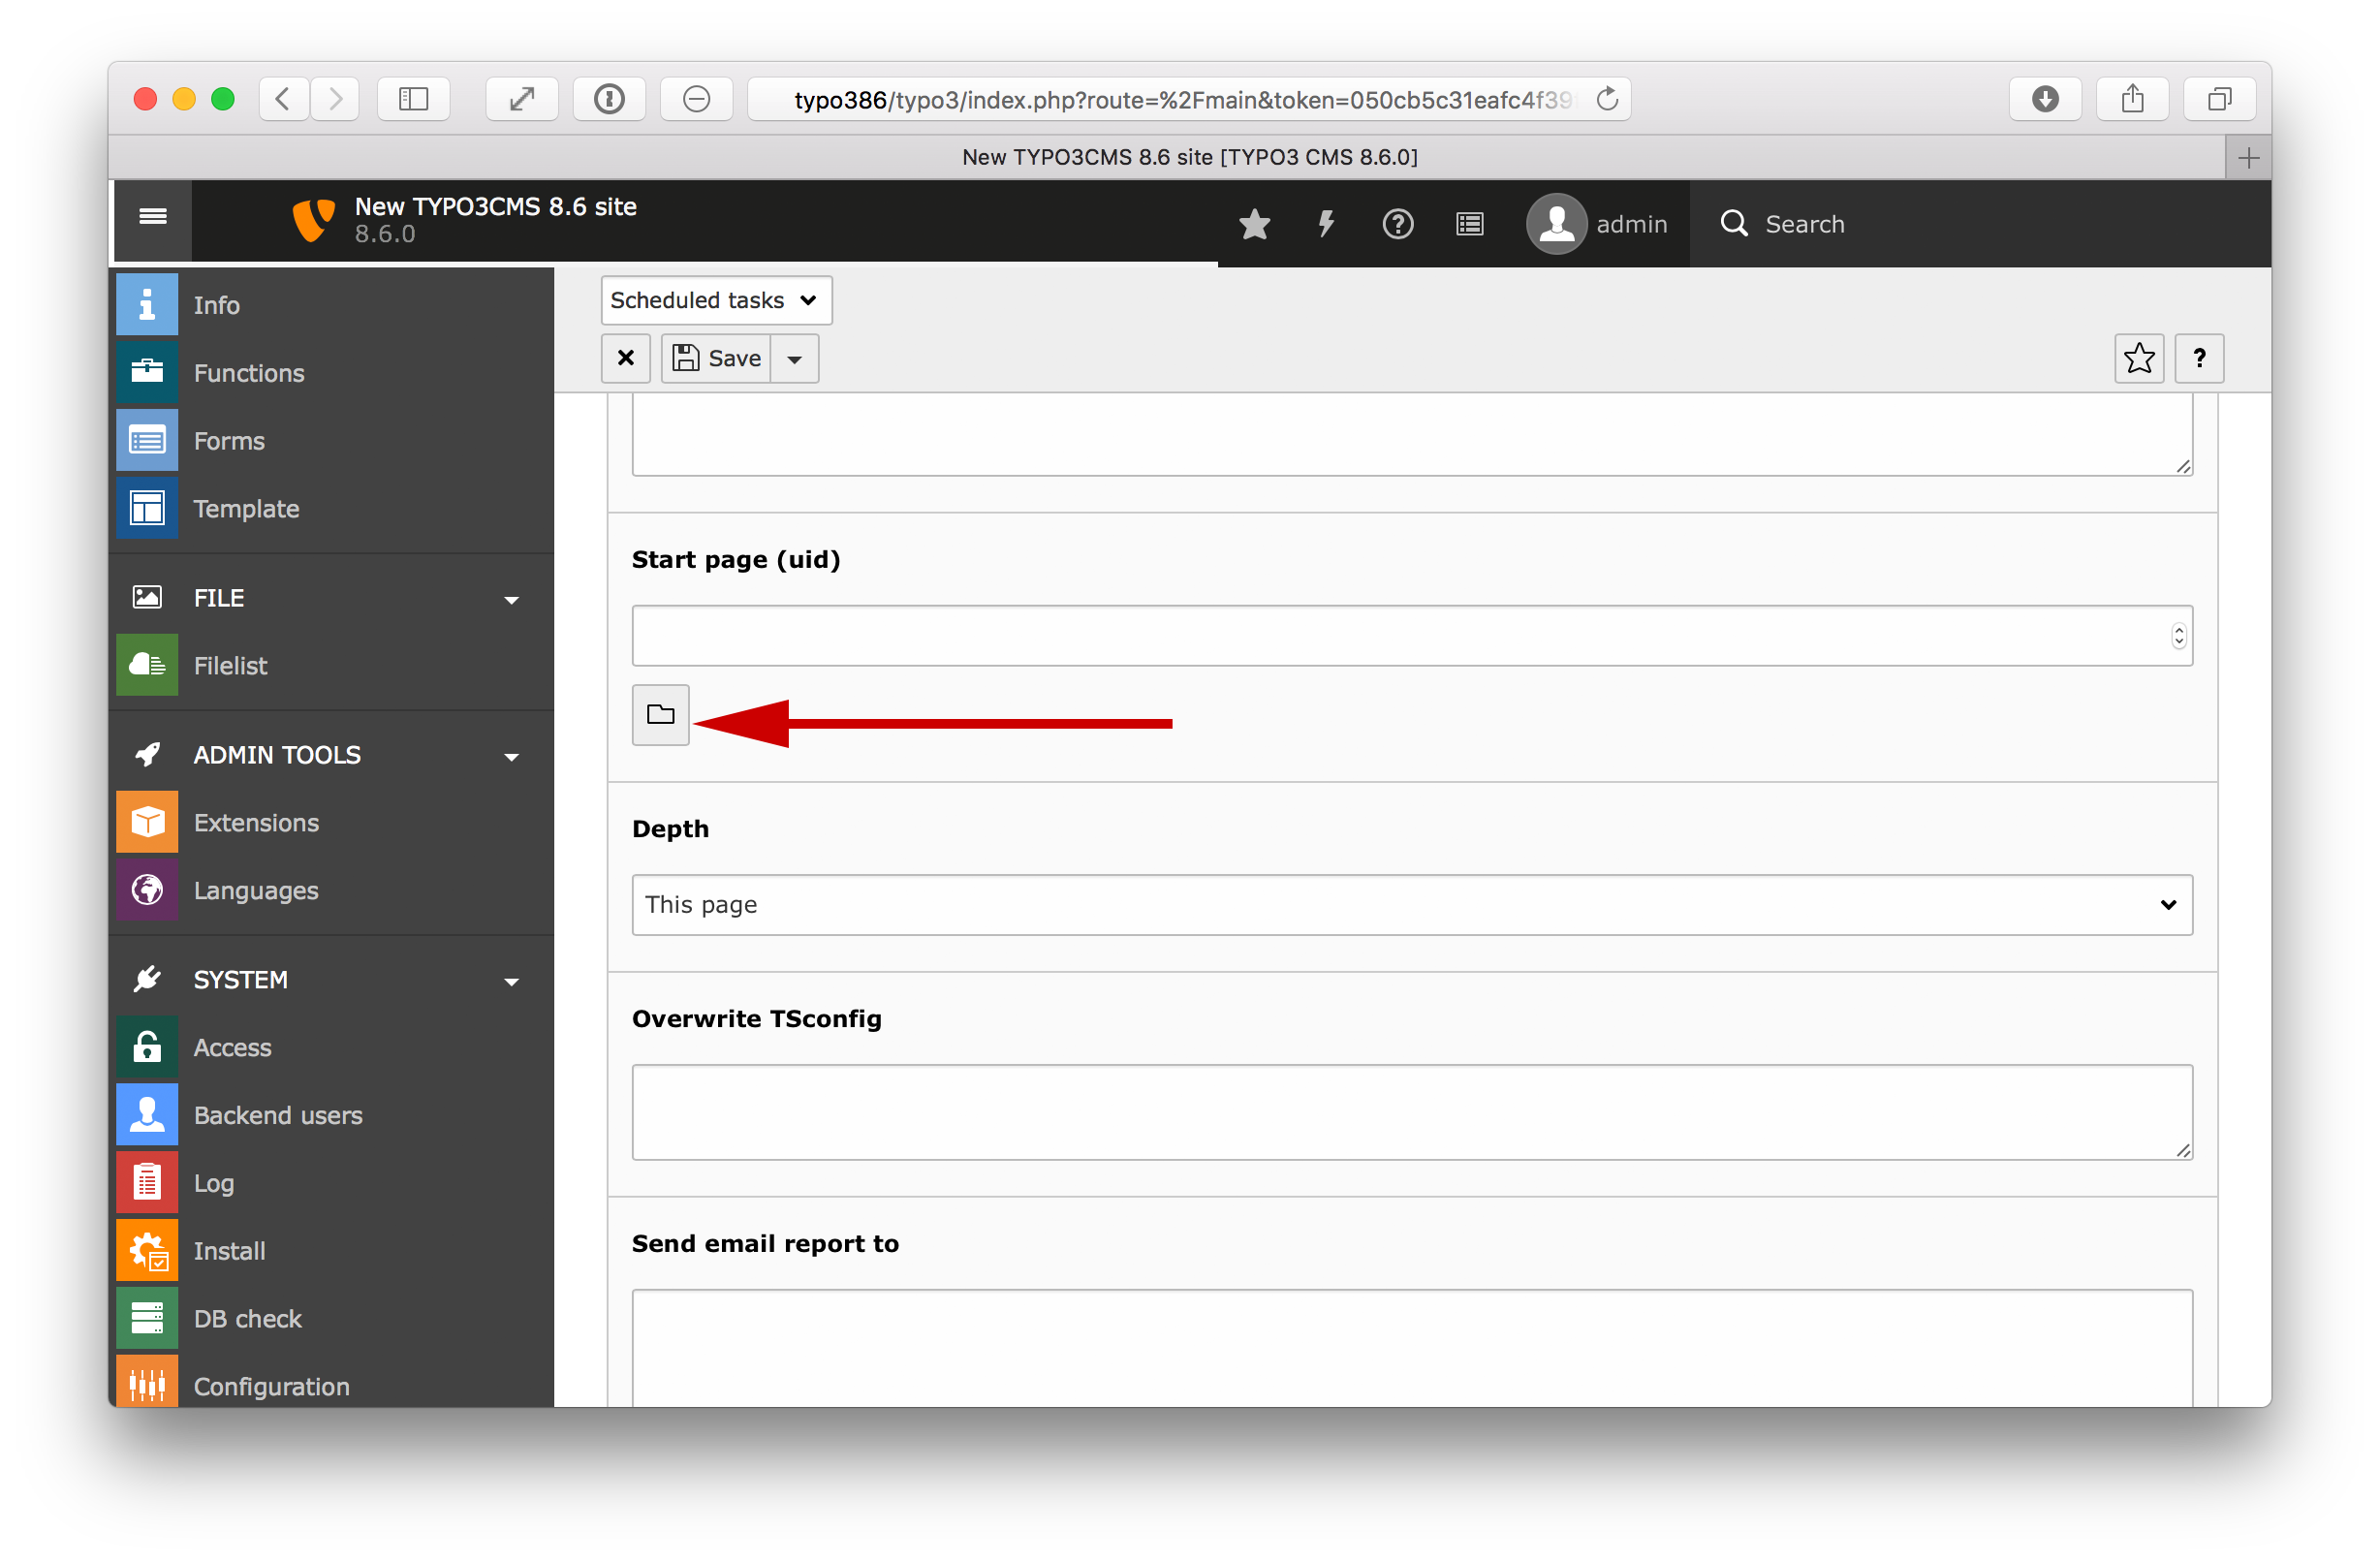
\includegraphics[width=0.67\linewidth]{BackendUserInterface/12211.png}
	\end{figure}

\end{frame}

% ------------------------------------------------------------------------------
% LTXE-SLIDE-START
% LTXE-SLIDE-UID:		0bd9b7d9-ac5c3bcf-e84f6b94-2857ef61
% LTXE-SLIDE-ORIGIN:	f924be39-75ae40d9-ba00f0a8-3a6de040 English
% LTXE-SLIDE-TITLE:		#45537: Manually executed tasks
% LTXE-SLIDE-REFERENCE:	!Feature: #45537 - Run manually executed tasks on next cron-run
% ------------------------------------------------------------------------------
\begin{frame}[fragile]
	\frametitle{Interfaccia utente Backend}
	\framesubtitle{Esecuzione dell'operazione, in funzionamento manuale, al successivo Cron-run}

	\begin{columns}[T]
		\begin{column}{0.35\textwidth}
			E' presente una nuova icona per selezionare un operazione da eseguire dal cron.
			Un nuovo bottone "Esegui le operazioni selezionate al prossimo cron job" è stato aggiunto, per
			marcare tutte le operazioni da eseguire al successivo cron job.
		\end{column}

		\begin{column}{0.65\textwidth}
			\begin{figure}\vspace{-0.6cm}
				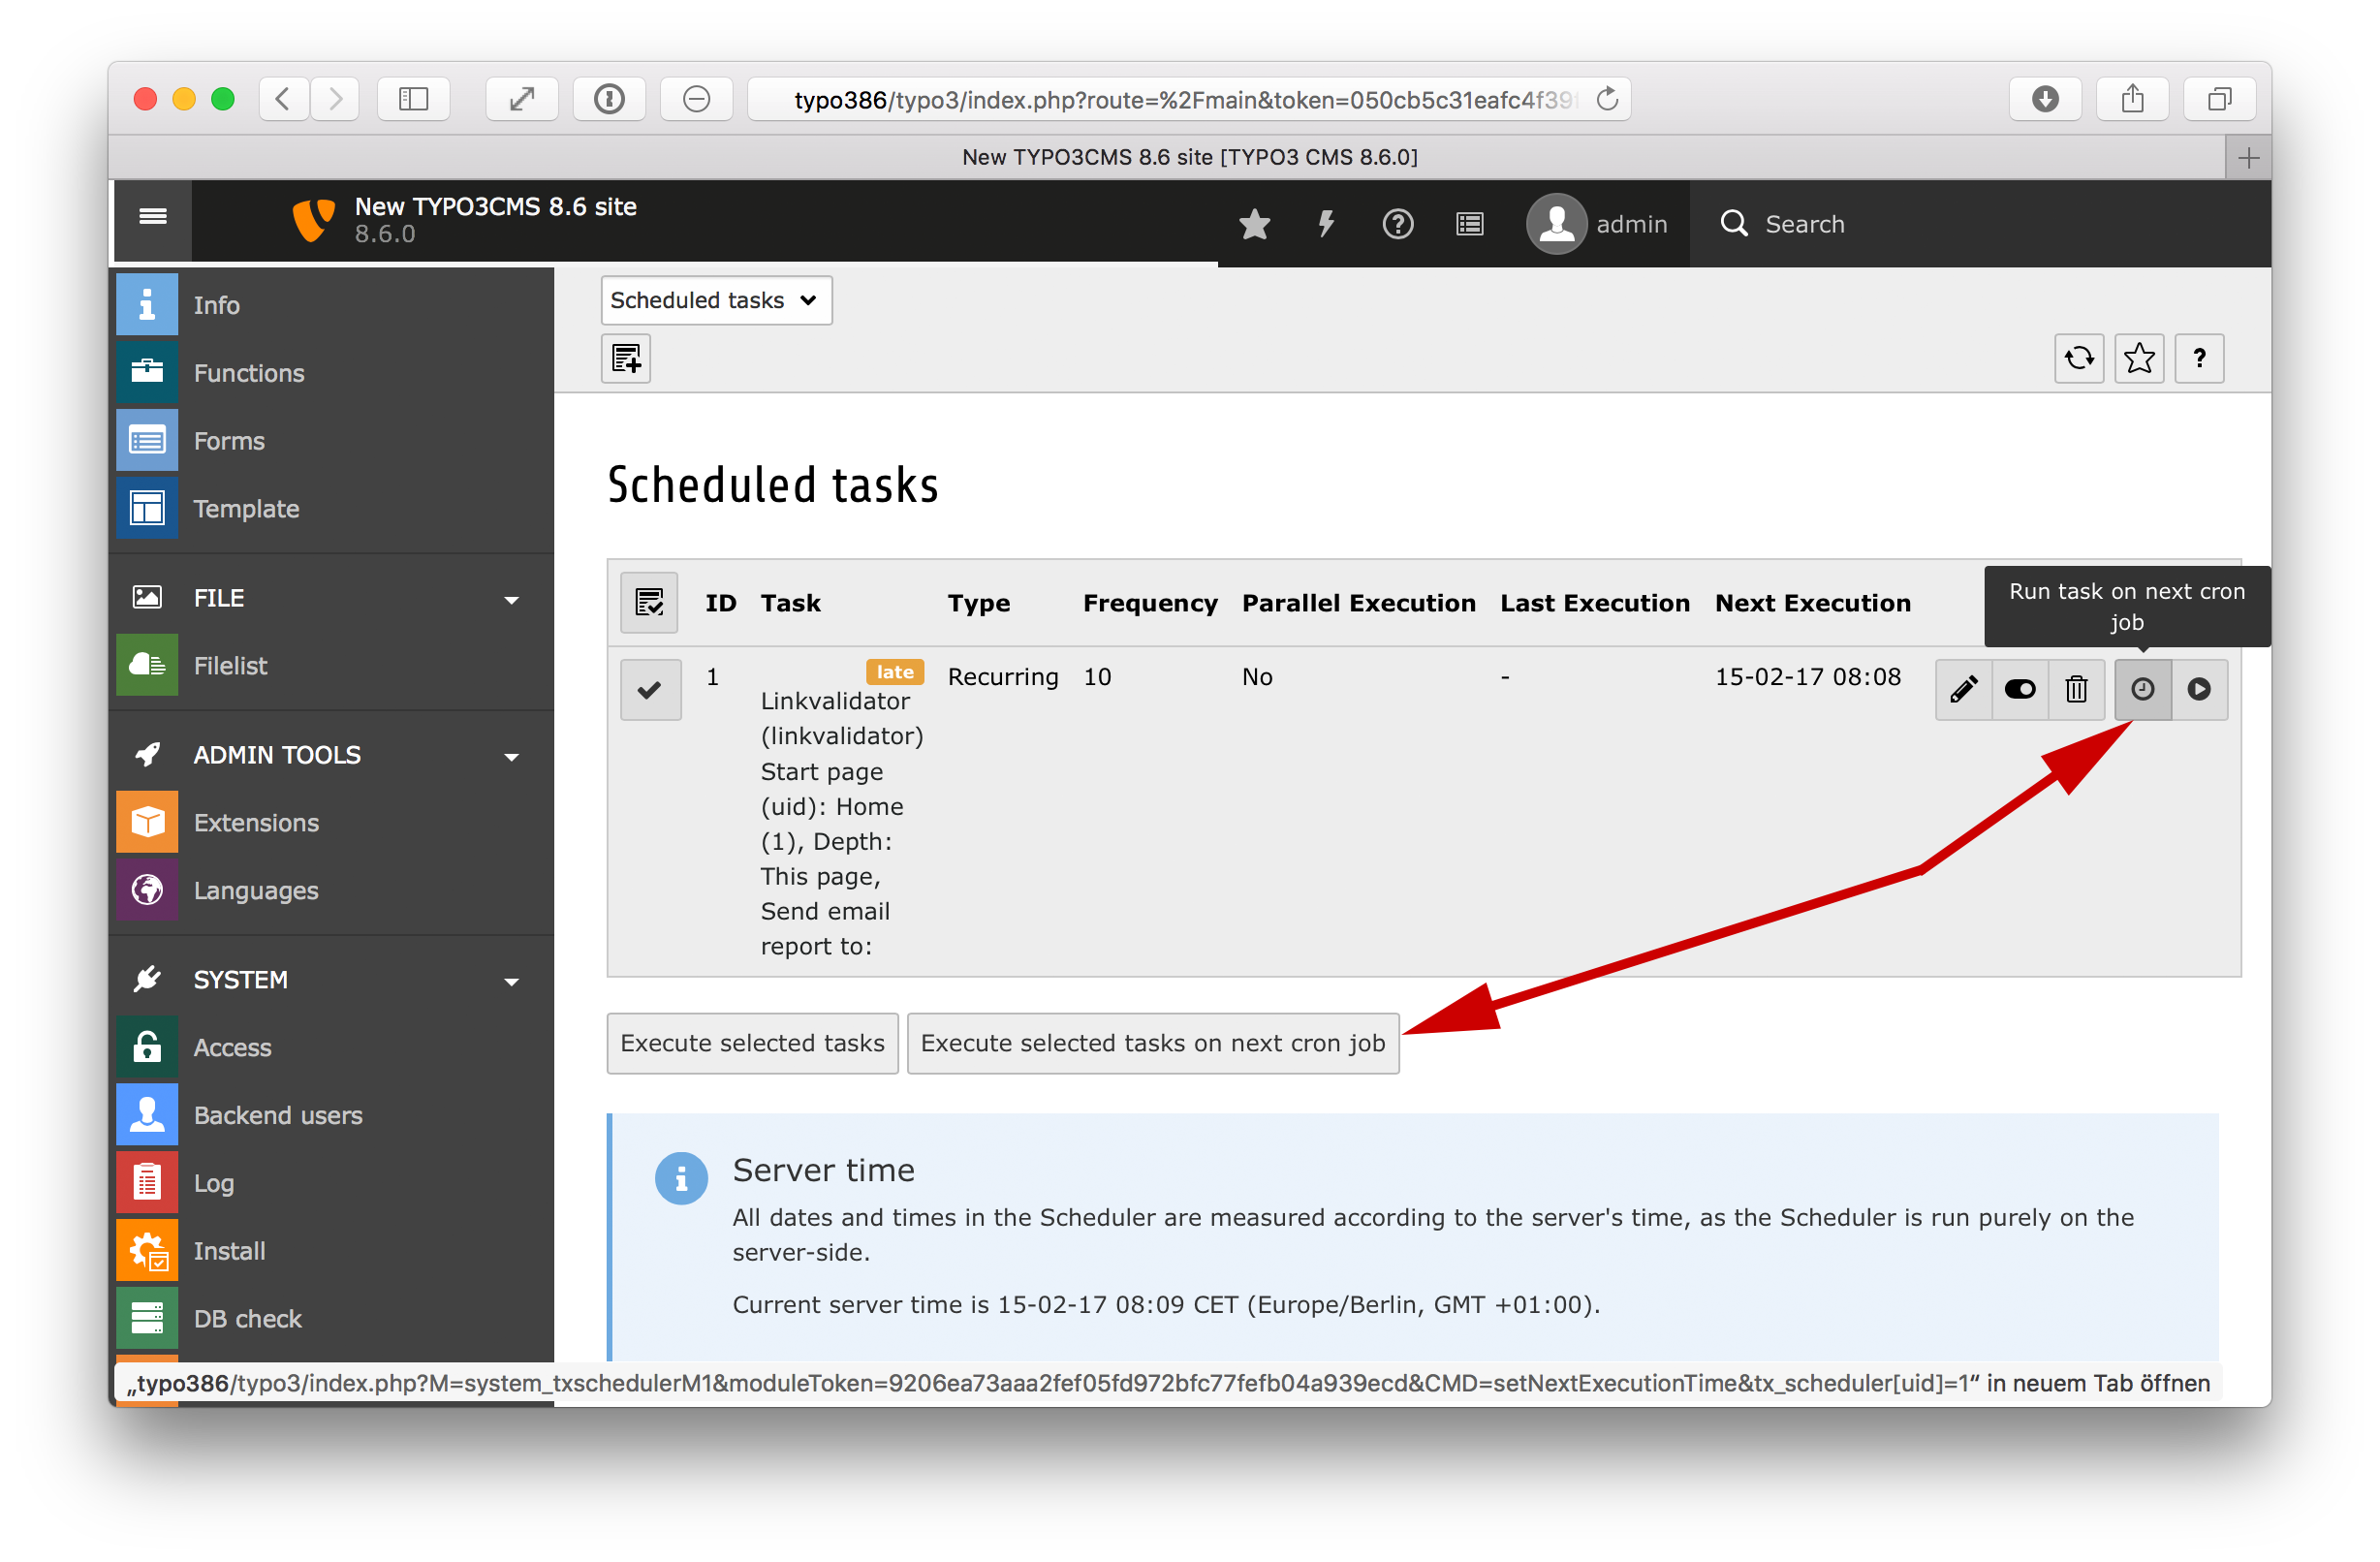
\includegraphics[width=0.99\linewidth]{BackendUserInterface/45537.png}
			\end{figure}
		\end{column}
	\end{columns}

\end{frame}

% ------------------------------------------------------------------------------
% LTXE-SLIDE-START
% LTXE-SLIDE-UID:		77901c40-c7a4c41a-ef91c942-c6f3427e
% LTXE-SLIDE-ORIGIN:	b6d6054e-21291d35-479a0095-a6e82a4f English
% LTXE-SLIDE-TITLE:		#47135: Paste Icon and Modal
% LTXE-SLIDE-REFERENCE:	!Feature: #51291 - Synchronized field values in localized records
% ------------------------------------------------------------------------------
\begin{frame}[fragile]
	\frametitle{Interfaccia utente Backend}
	\framesubtitle{Icona incolla e conferma modale}

	Quando la clipboard normale contiene un elemento, un icona incolla diventa attiva
	nella pagina modulo. Quando l'utente clicca sull'icona, un messaggio modale appare per 
	avere conferma dall'utente dell'azione.

	\begin{figure}\vspace{-0.2cm}
		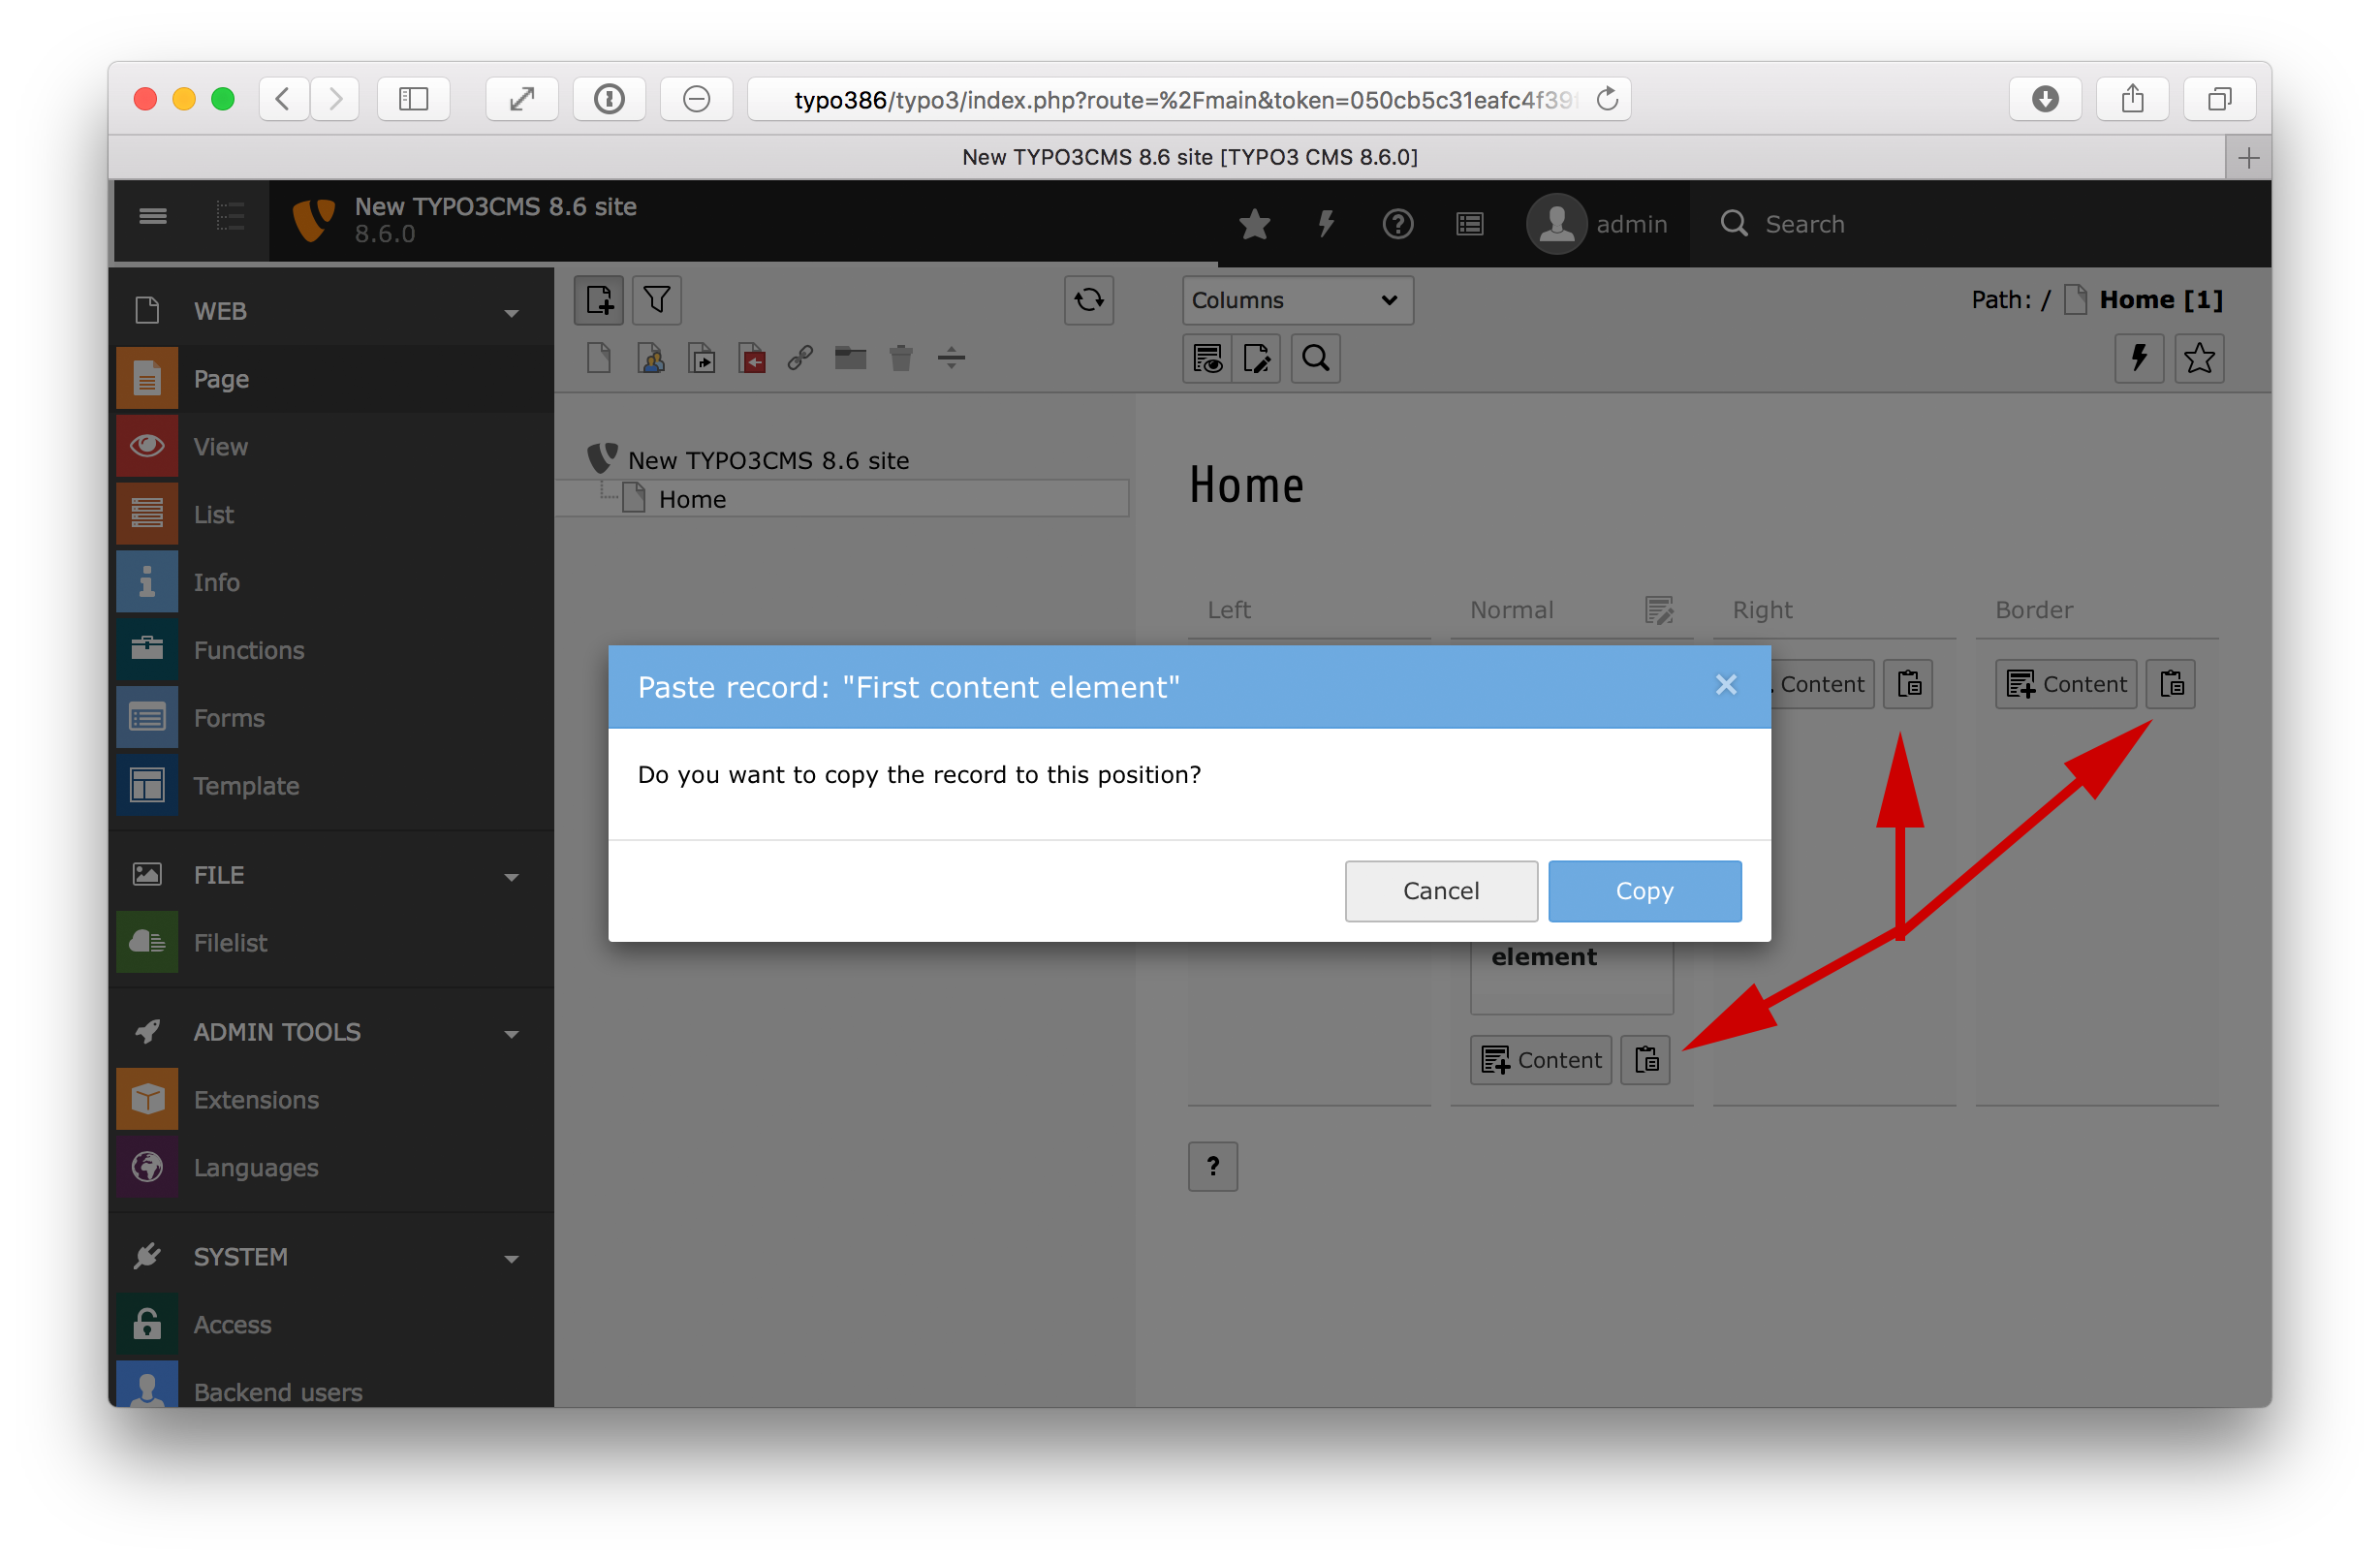
\includegraphics[width=0.63\linewidth]{BackendUserInterface/47135.png}
	\end{figure}

\end{frame}

% ------------------------------------------------------------------------------
% LTXE-SLIDE-START
% LTXE-SLIDE-UID:		f1361b55-1012651b-bbb613a7-12840bec
% LTXE-SLIDE-ORIGIN:	b31e455f-fce042ed-e3670436-9e72983c English
% LTXE-SLIDE-TITLE:		#67243: Folding of Scheduler Task Groups
% LTXE-SLIDE-REFERENCE:	!Feature: #67243 - Implement folding of scheduler task groups
% ------------------------------------------------------------------------------
\begin{frame}[fragile]
	\frametitle{Interfaccia utente Backend}
	\framesubtitle{Sezione con gruppi attività schedulate}

	Quando si utilizzano gruppi di lavoro, le attività sono visualizzate nella lista dei gruppi di attività.
	Cliccando sulla riga con il titolo del gruppo, viene nascosto o mostrato l'elenco delle attività.

	\begin{figure}\vspace{-0.3cm}
		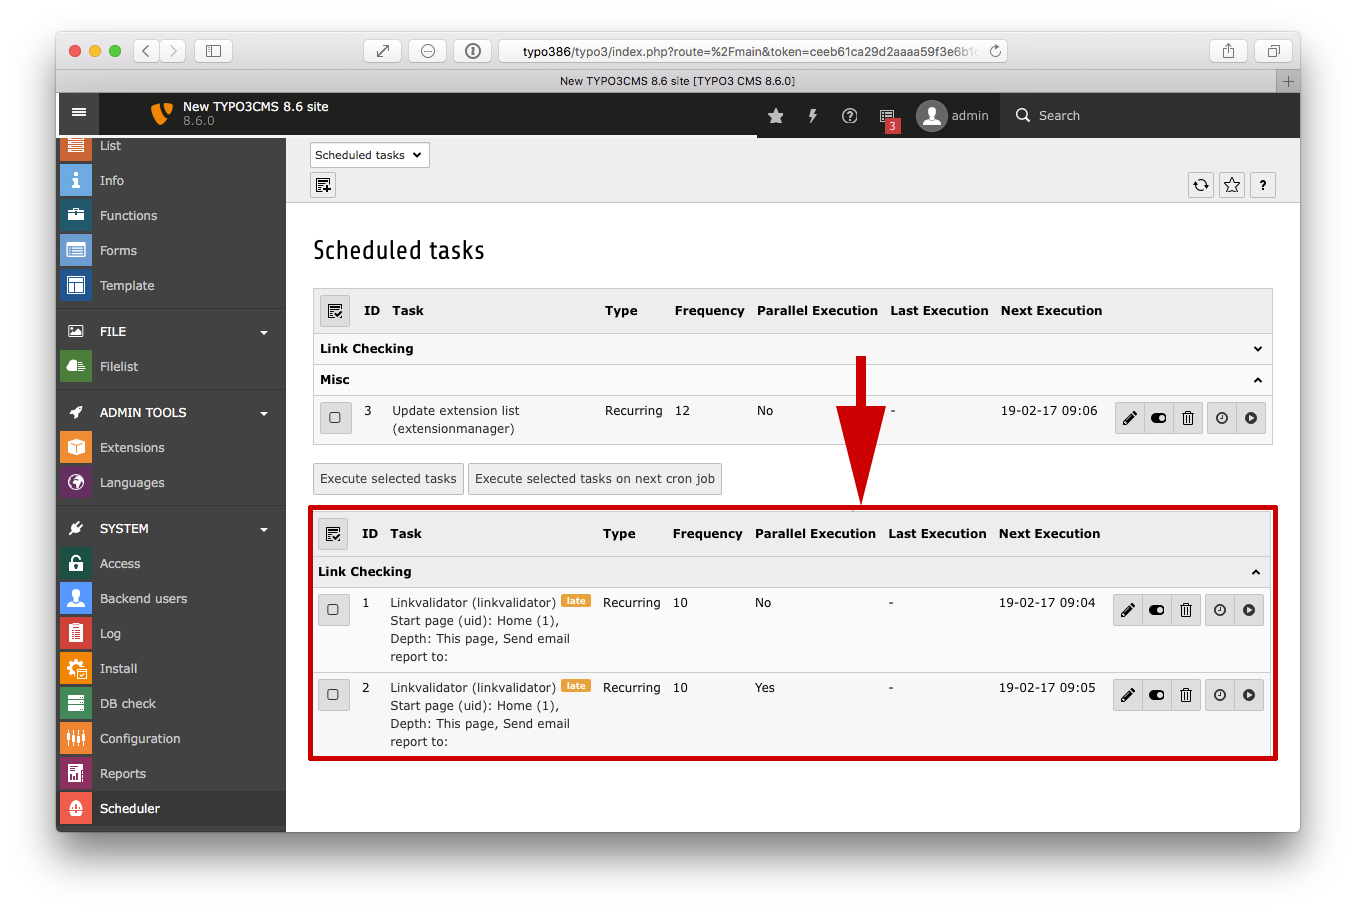
\includegraphics[width=0.60\linewidth]{BackendUserInterface/67243.png}
	\end{figure}

\end{frame}

% ------------------------------------------------------------------------------
% LTXE-SLIDE-START
% LTXE-SLIDE-UID:		4baabc6c-7b400605-0bc4ae71-2e8e1a95
% LTXE-SLIDE-ORIGIN:	14fe5a0b-2a22a6ce-325b5de1-ef26ce50 English
% LTXE-SLIDE-TITLE:		#69572: Page Module Notice
% LTXE-SLIDE-REFERENCE:	!Feature: #69572 - Page module Notice "Content is also shown on:"
% ------------------------------------------------------------------------------
\begin{frame}[fragile]
	\frametitle{Interfaccia utente Backend}
	\framesubtitle{Avviso nel modulo Pagina "Il contenuto è visualizzato anche in"}

	\begin{columns}[T]
		\begin{column}{.3\textwidth}
			Quando il contenuto della pagina viene visualizzato anche su una pagina diversa via	
			"Mostra contenuto dalla pagina", viene visualizzato un avviso sulla pagina che sta
			fornendo il contenuto ad una pagina differente.
		\end{column}

		\begin{column}{.7\textwidth}
			\begin{figure}\vspace*{-0.6cm}
				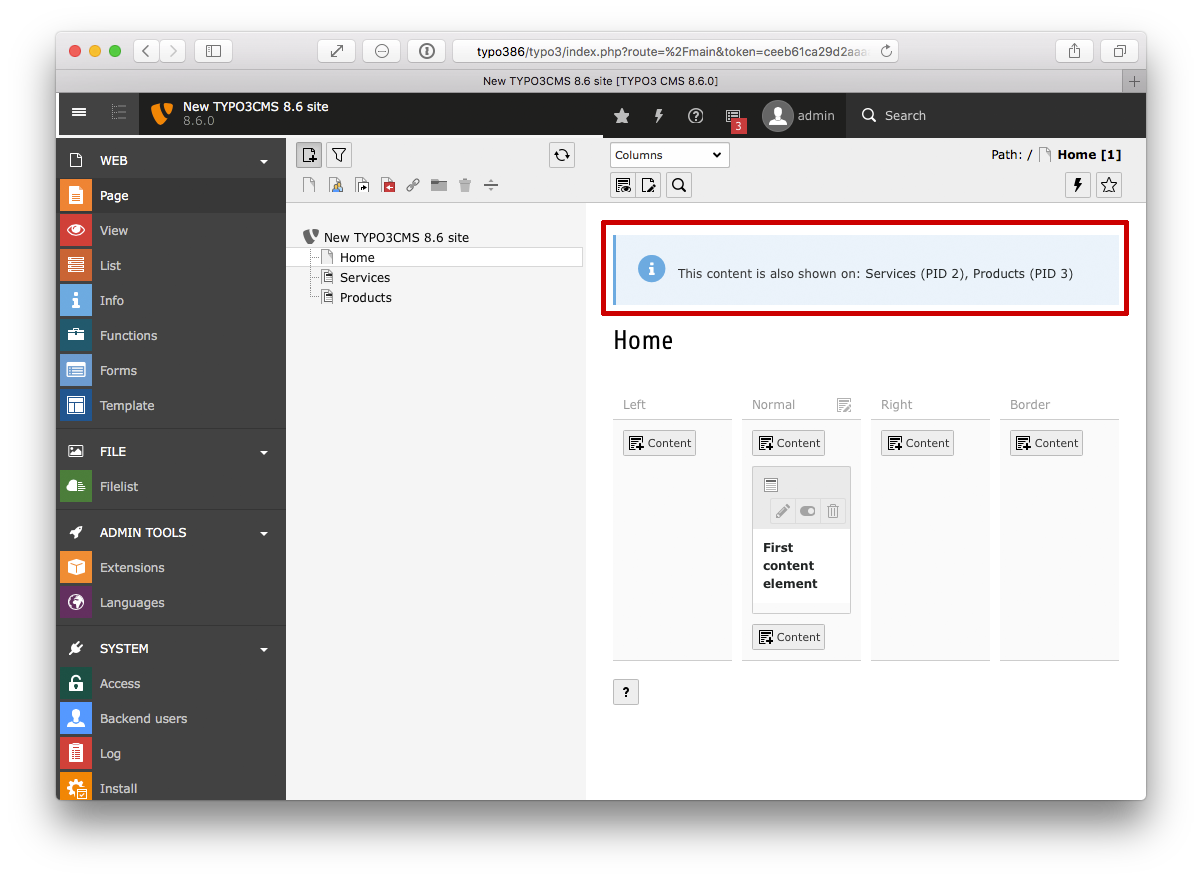
\includegraphics[width=\linewidth]{BackendUserInterface/69572.png}
			\end{figure}
		\end{column}
	\end{columns}

\end{frame}

% ------------------------------------------------------------------------------
% LTXE-SLIDE-START
% LTXE-SLIDE-UID:		01120430-e15fd8cc-df1ee468-ebec3ee9
% LTXE-SLIDE-ORIGIN:	23a4baef-462e7d0c-c8cd4cfc-9dac1f99 English
% LTXE-SLIDE-TITLE:		#75880: Image Manipulation - Multiple Cropping Variants
% LTXE-SLIDE-REFERENCE:	!Feature: #75880 - Implement multiple cropping variants in image manipulation tool
% ------------------------------------------------------------------------------
\begin{frame}[fragile]
	\frametitle{Interfaccia utente Backend}
	\framesubtitle{Manipolazione immagini - Varianti multiple di ritaglio}

	Lo strumento di manipolazione delle immagini è ora in grado di gestire più varianti di ritaglio (se configurato).
	Gli utenti posso selezionare un'area di focus, dentro l'area ritagliata, indicando l'area dell'immagine che
	deve essere visibile per mantenere il significato dell'immagine.
	
	\begin{columns}[T]
		\begin{column}{.4\textwidth}
			Per dare un suggerimento ai redattori sull'area dell'immagine che viene utilizzata da altri elementi 
			del DOM come i titoli, quando si seleziona un area di ritaglio, è possibile definire più aree di copertura.
		\end{column}

		\begin{column}{.6\textwidth}
			\begin{figure}\vspace*{-0.6cm}
				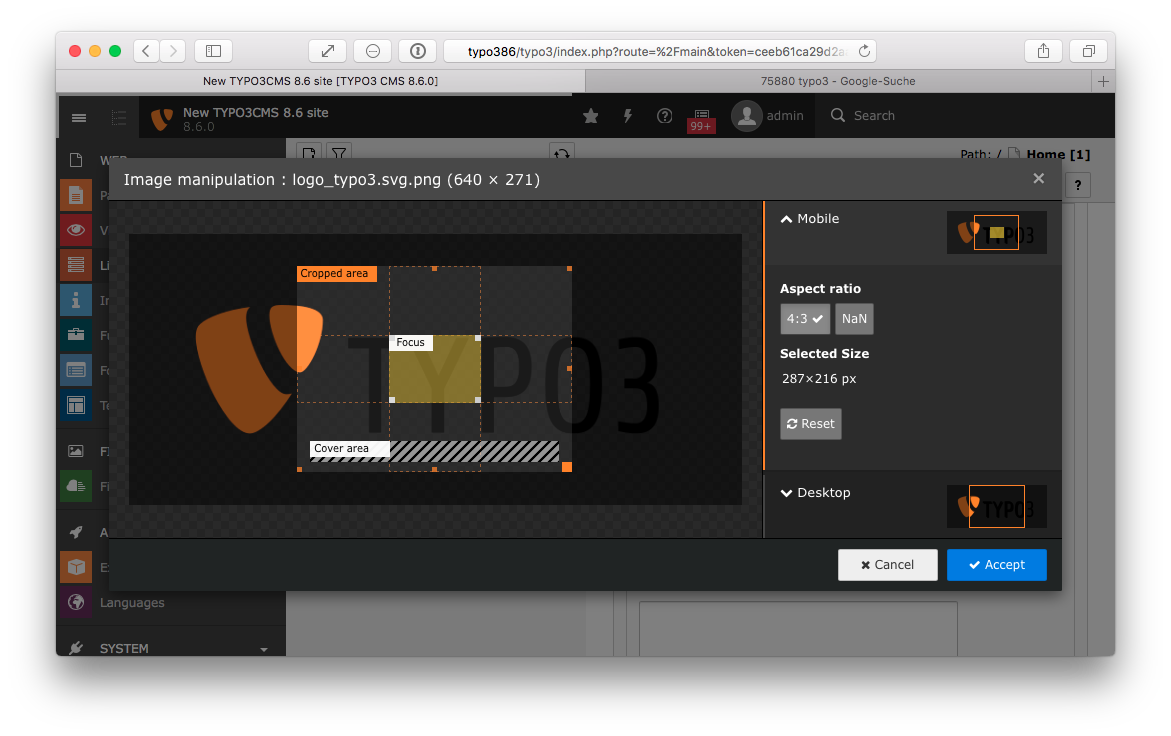
\includegraphics[width=0.99\linewidth]{BackendUserInterface/75880.png}
			\end{figure}
		\end{column}
	\end{columns}

\end{frame}

% ------------------------------------------------------------------------------
% LTXE-SLIDE-START
% LTXE-SLIDE-UID:		ed22c502-cb6ad578-9c2a3205-728ae8d2
% LTXE-SLIDE-ORIGIN:	8f2f695d-f5c6a8bf-5700cf34-d6389ce8 English
% LTXE-SLIDE-TITLE:		#79235: Delete Similar Errors (sys_log)
% LTXE-SLIDE-REFERENCE:	!Feature: #79235 - Add button to delete similar errors from sys_log
% ------------------------------------------------------------------------------
\begin{frame}[fragile]
	\frametitle{Interfaccia utente Backend}
	\framesubtitle{Cancellare errori simili nel \texttt{sys\_log}}
	
	Il modulo di log di TYPO3 dispone ora di un pulsante per cancellare errori multipli in una sola volta
	sulla base del campo \texttt{dettagli} della tabella \texttt{sys\_log}. Questo è utile quando
	viene corretto un errore con molte voci nel registro.

	\begin{figure}\vspace{-0.2cm}
		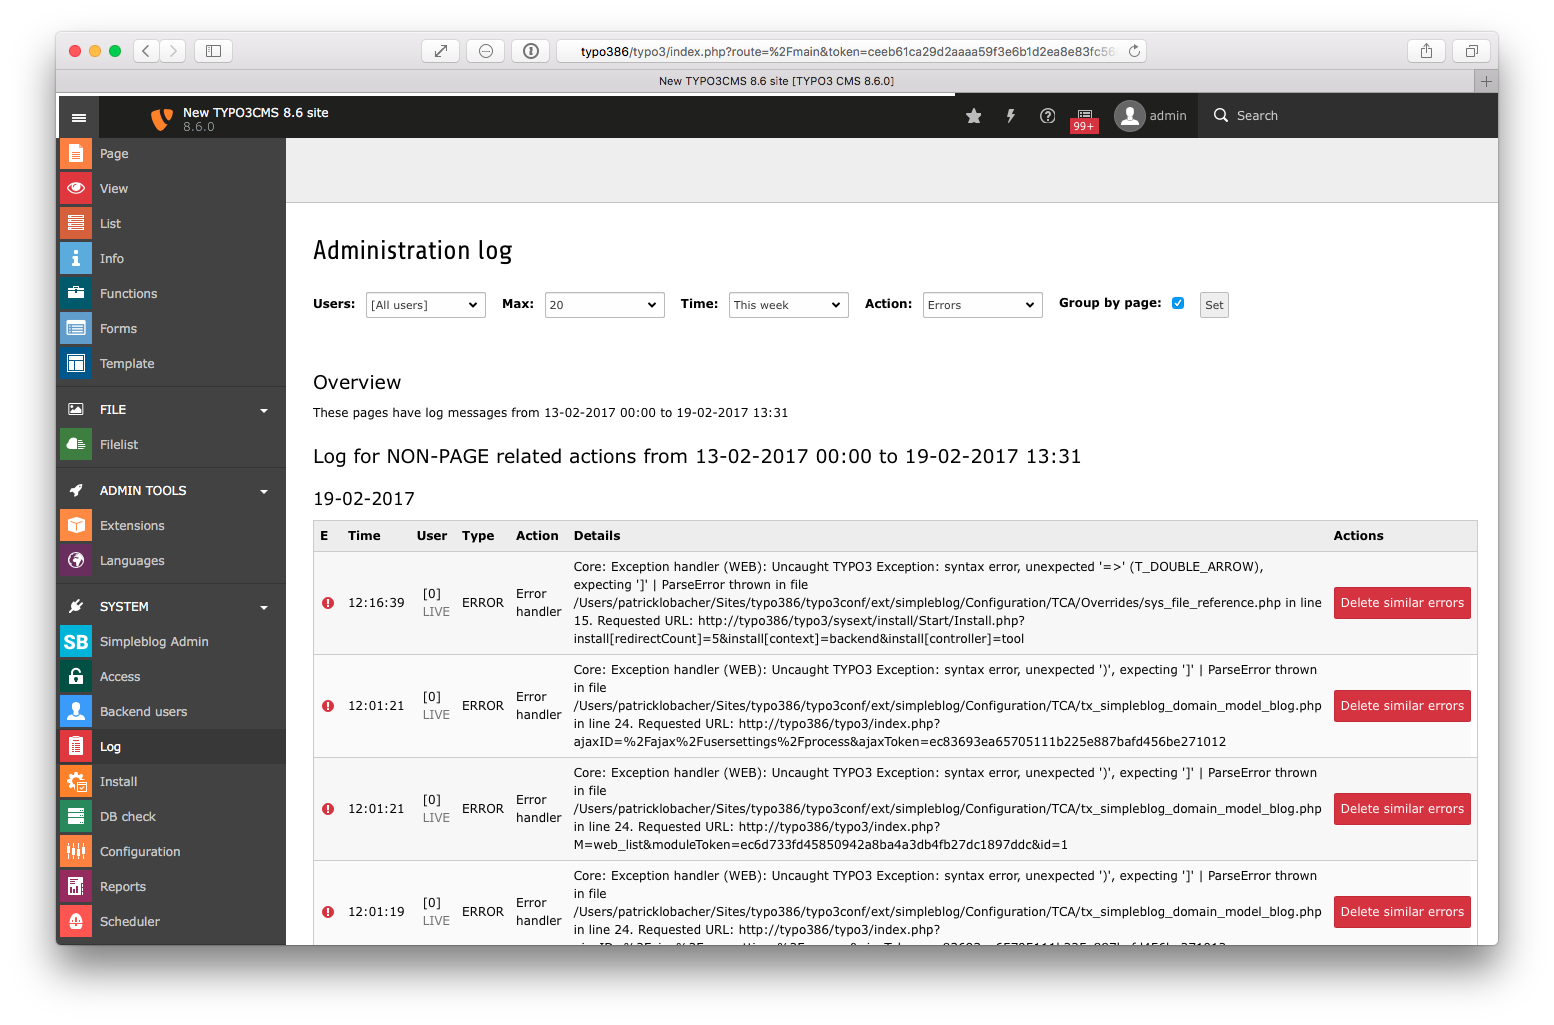
\includegraphics[width=0.60\linewidth]{BackendUserInterface/79235.png}
	\end{figure}

\end{frame}

% ------------------------------------------------------------------------------
% LTXE-SLIDE-START
% LTXE-SLIDE-UID:		5bfb81d5-60fc8d7f-2120c090-35f3d6e8
% LTXE-SLIDE-ORIGIN:	fc878ad9-7b163d51-e579b8b3-9cbe41d9 English
% LTXE-SLIDE-TITLE:		#79467: Form settings button
% LTXE-SLIDE-REFERENCE:	!Feature: #79467 - EXT:form - add form settings button to module header
% ------------------------------------------------------------------------------
\begin{frame}[fragile]
	\frametitle{Interfaccia utente Backend}
	\framesubtitle{\texttt{EXT:form}: bottone di modifica impostazioni del form nell’intestazione del modulo}

	Un nuovo pulsante è stato aggiunto nell'header del modulo dell'editor dei form.
	Cliccando su questo bottone sono mostrate le impostazioni del modulo in una sezione di ispezione.

	\begin{figure}\vspace{-0.2cm}
		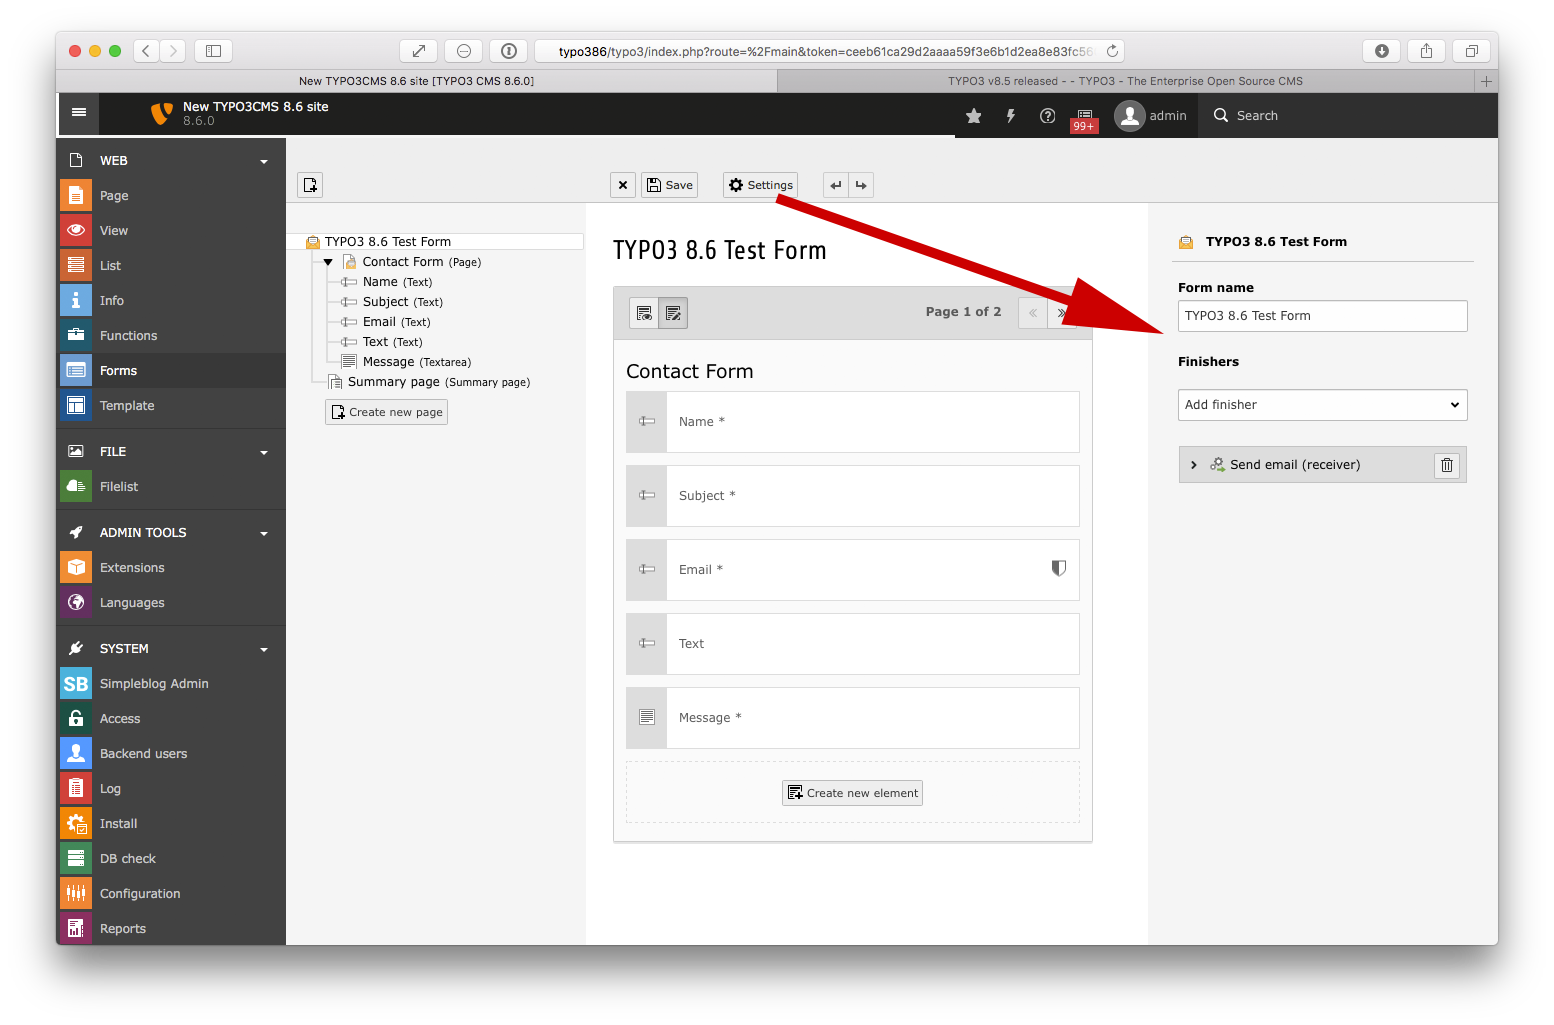
\includegraphics[width=0.675\linewidth]{BackendUserInterface/79467.png}
	\end{figure}

\end{frame}

% ------------------------------------------------------------------------------
% LTXE-SLIDE-START
% LTXE-SLIDE-UID:		a2511ebf-acf21976-a2d7c258-db38861b
% LTXE-SLIDE-ORIGIN:	e1759d2e-8cc138ca-40ce6a34-65354b0e English
% LTXE-SLIDE-TITLE:		#79531: EXT:form - Add multiselect inspector editor
% LTXE-SLIDE-REFERENCE:	!Feature: #79531 - EXT:form - Add multiselect inspector editor
% ------------------------------------------------------------------------------
\begin{frame}[fragile]
	\frametitle{Interfaccia utente Backend}
	\framesubtitle{{EXT:form}: Aggiunta una sezione di ispezione multiselect}

	\begin{columns}[T]
		\begin{column}{0.4\textwidth}
			E' stato aggiunto un nuovo campo nell'editor di form e nella sezione di ispezione.
			Se applicato, campi di selezione multipla possono essere aggiunti nell'inspector.
			Un campo di selezione multipla permette di selezionare più proprietà meta di un campo
			e le memorizza in un percorso di proprietà definita.
		\end{column}

		\begin{column}{0.6\textwidth}
			\begin{figure}\vspace*{-0.6cm}
				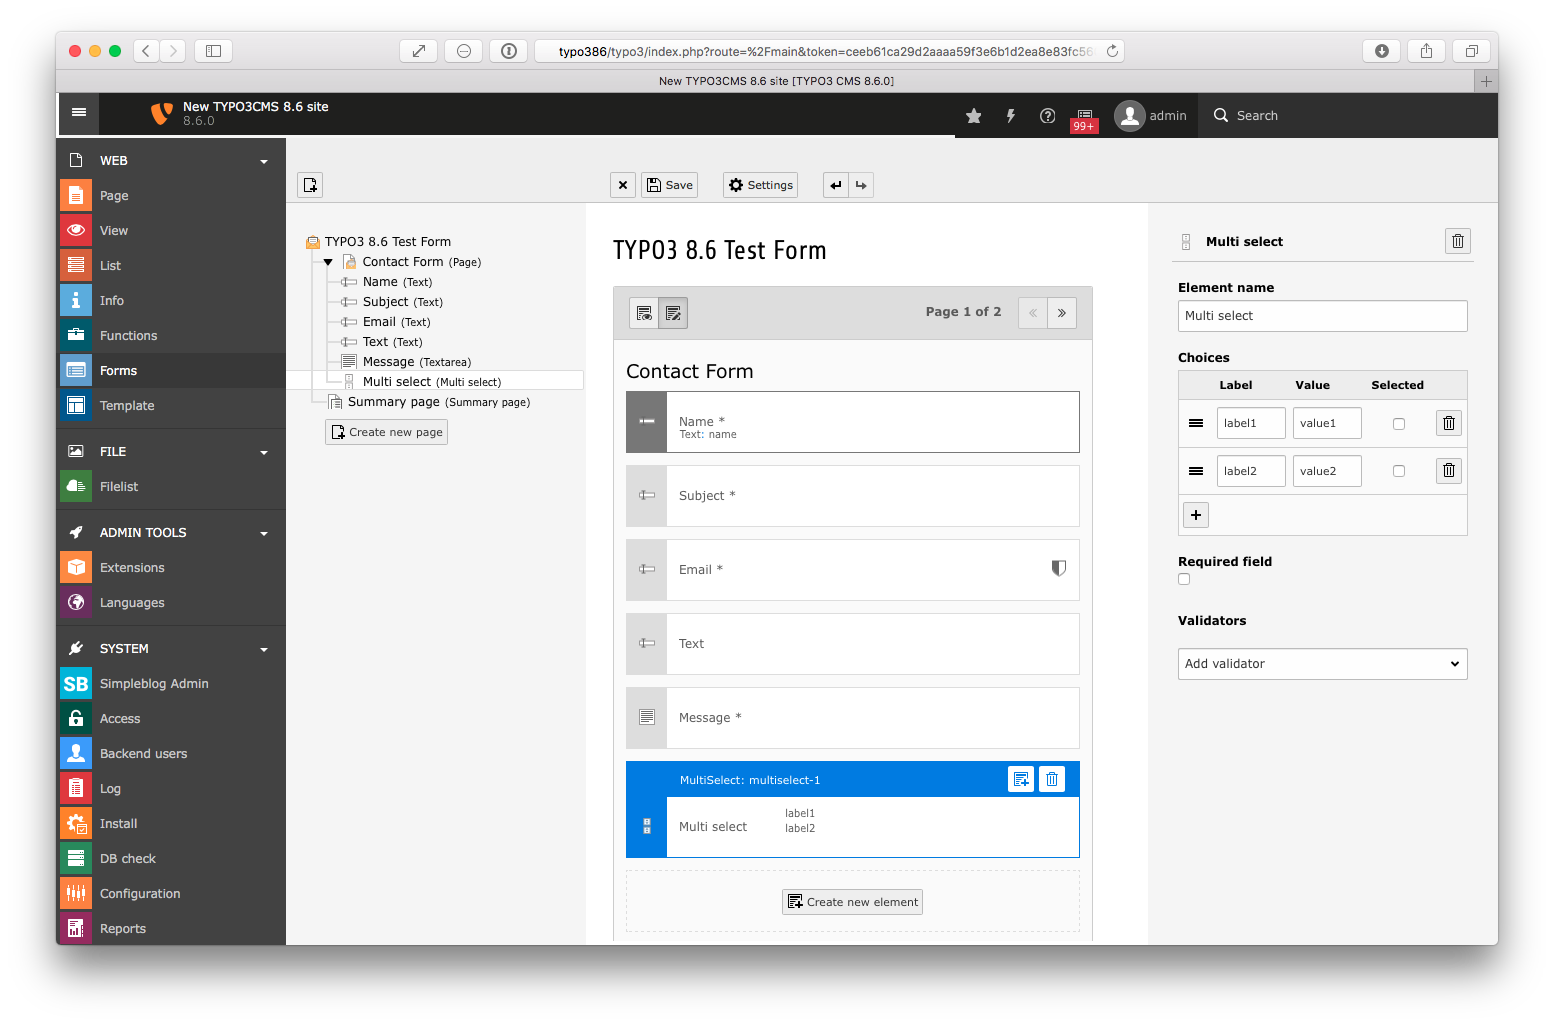
\includegraphics[width=0.99\linewidth]{BackendUserInterface/79531.png}
			\end{figure}
		\end{column}
	\end{columns}

\end{frame}

% ------------------------------------------------------------------------------
% LTXE-SLIDE-START
% LTXE-SLIDE-UID:		3914070e-21920b3b-edf7f8be-7bd60f42
% LTXE-SLIDE-ORIGIN:	f6756002-b9aac45f-9460b472-1da819b5 English
% LTXE-SLIDE-TITLE:		#79521: Show list of failed input elements in FormEngine
% LTXE-SLIDE-REFERENCE:	!Feature: #79521 - Show list of failed input elements in FormEngine
% ------------------------------------------------------------------------------
\begin{frame}[fragile]
	\frametitle{Interfaccia utente Backend}
	\framesubtitle{Vista della lista di elementi di input errati nel FormEngine}

	\begin{columns}[T]
		\begin{column}{.45\textwidth}
			Se durante la convalida dei campi di input nel FormEngine ci sono degli errori, un pulsante
			viene mostrato nella barra dei pulsanti nell'intestazione del modulo dei documenti.
			Cliccando sul pulsante è mostrato un elenco con tutti gli elementi di input la cui validazione
			è fallita. Cliccando sul campo nell'elenco viene evidenziato automaticamente il campo nel form.
		\end{column}

		\begin{column}{.55\textwidth}
			\begin{figure}\vspace*{-0.6cm}
				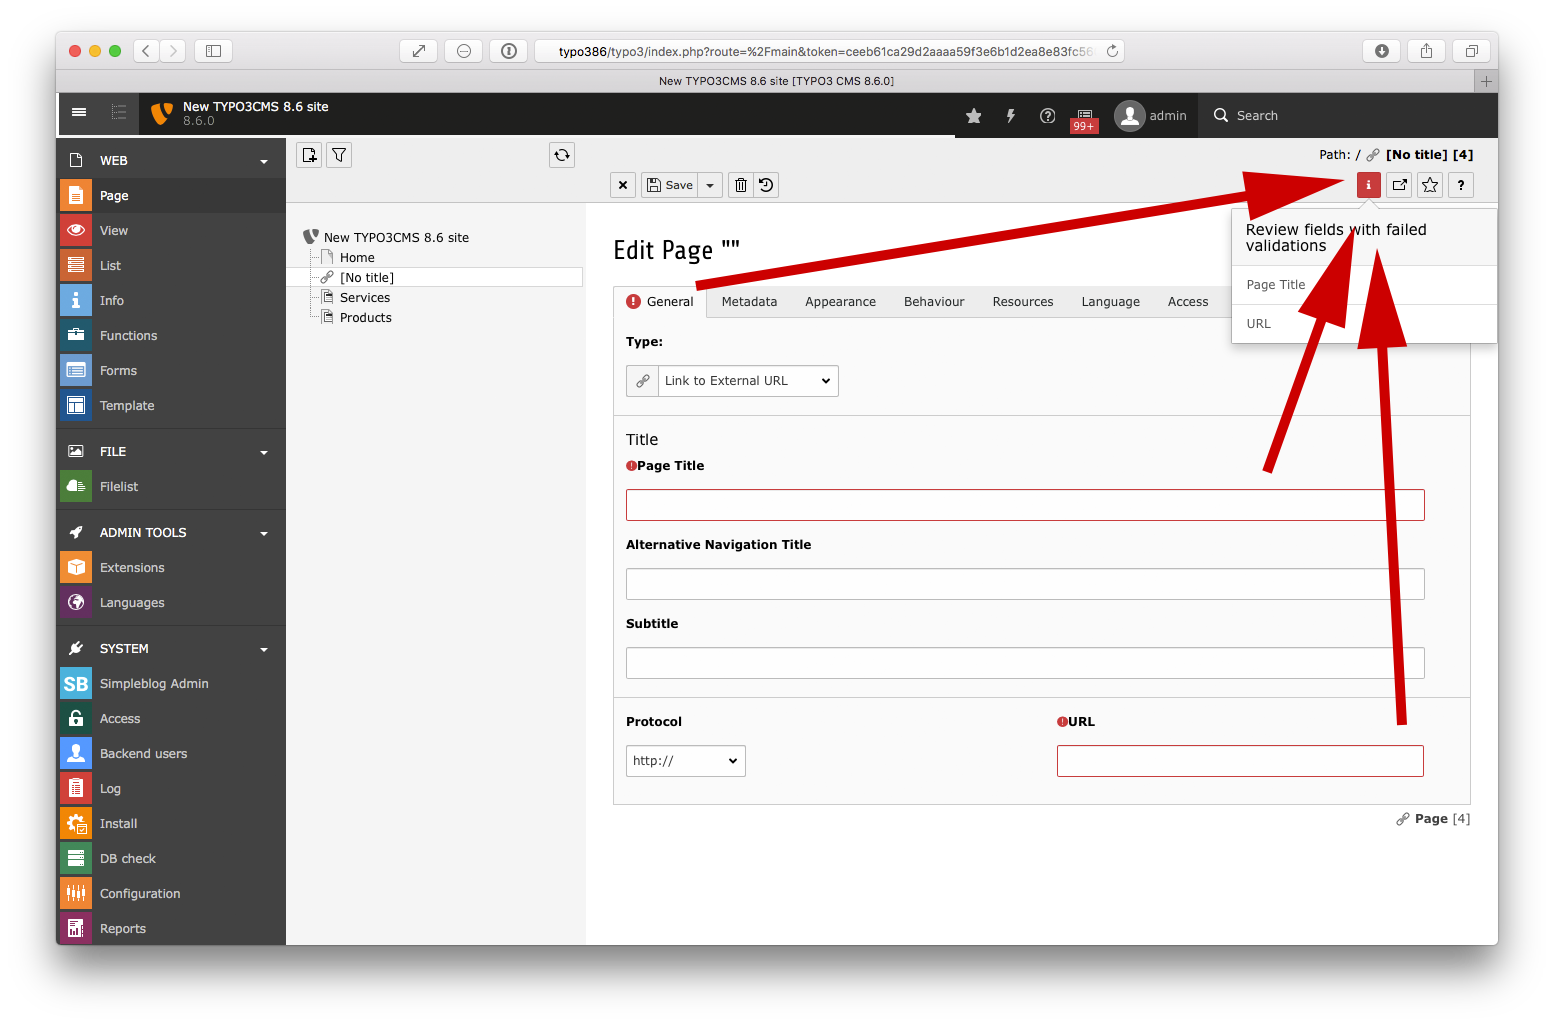
\includegraphics[width=0.99\linewidth]{BackendUserInterface/79521.png}
			\end{figure}
		\end{column}
	\end{columns}

\end{frame}

% ------------------------------------------------------------------------------
% LTXE-SLIDE-START
% LTXE-SLIDE-UID:		54437a4b-ada75cd7-c419e453-1dc8f44b
% LTXE-SLIDE-ORIGIN:	749a055b-02003192-92f2631e-39abcc95 English
% LTXE-SLIDE-TITLE:		#79622: Dedicated content elements for menus
% LTXE-SLIDE-REFERENCE:	!Breaking: #79622 - Dedicated content elements for menus
% ------------------------------------------------------------------------------
\begin{frame}[fragile]
	\frametitle{Interfaccia utente Backend}
	\framesubtitle{Elementi di contenuto menu dedicati}

	Per una migliore manutenzione l'elemento di contenuto menu esistente è stato suddiviso 
	in più elementi di contenuto dedicati

	\begin{figure}\vspace{-0.2cm}
		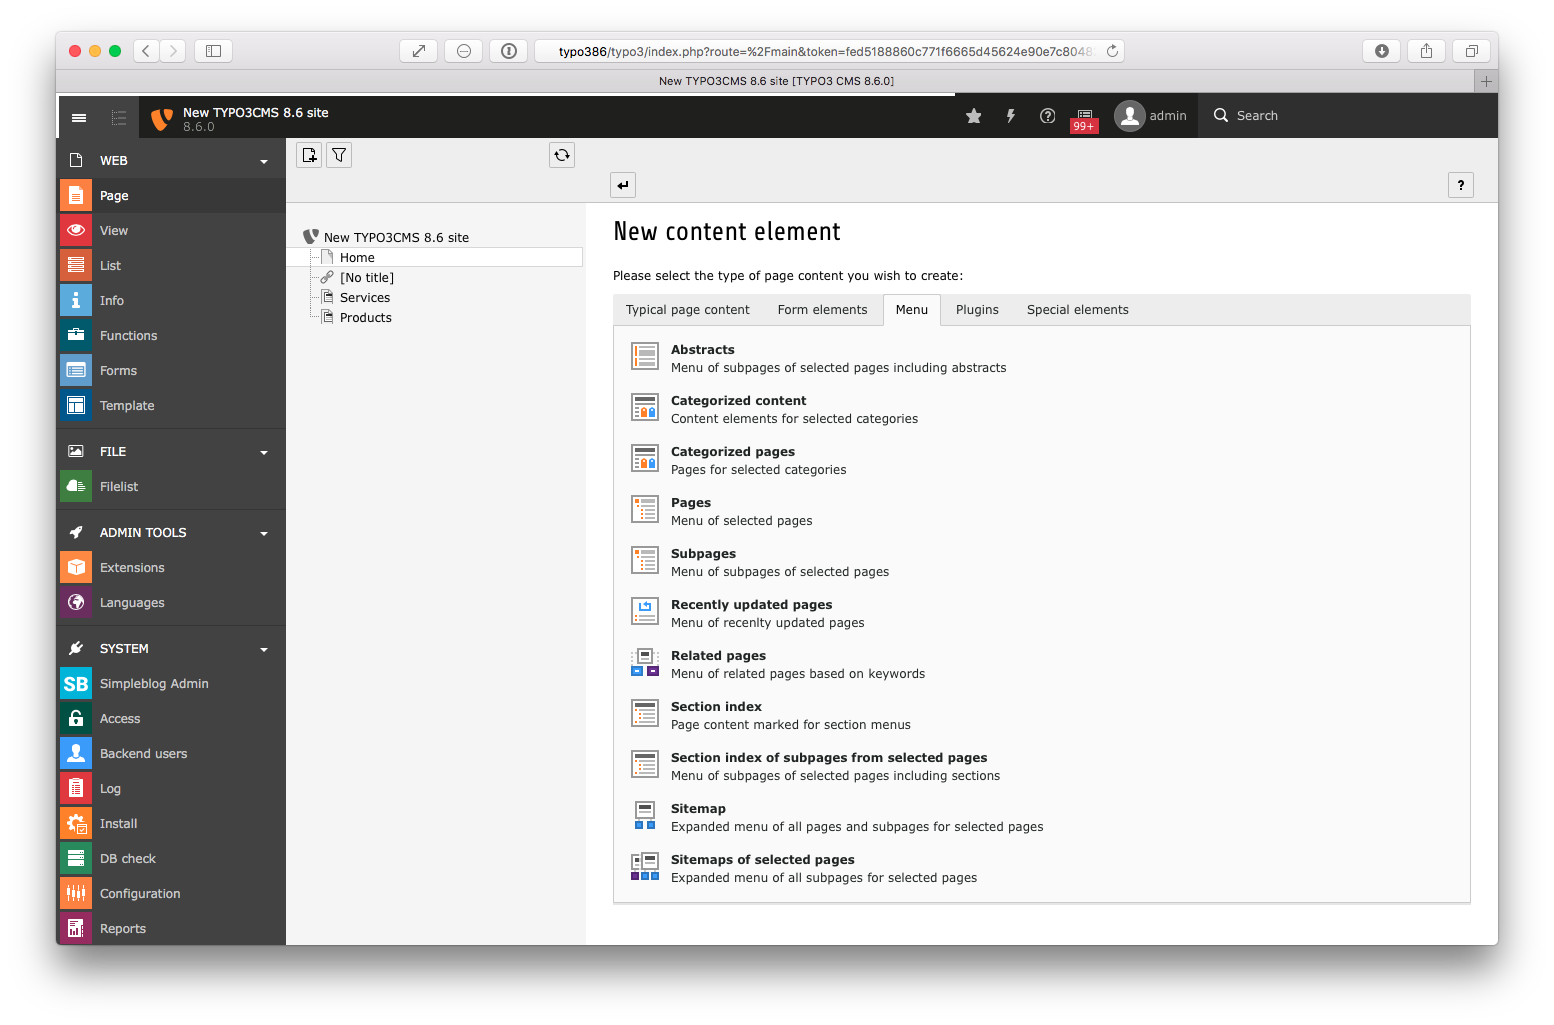
\includegraphics[width=0.68\linewidth]{BackendUserInterface/79622.png}
	\end{figure}

\end{frame}

% ------------------------------------------------------------------------------
